\documentclass[11pt]{article}
% Shared preamble for the AmberMeta SOP and its companion note.
%
% Deliberately confined to what ships with a distro TeX Live (no tlmgr on the
% workstation these are built on): every package below is in texlive-latex-recommended
% or texlive-fonts-recommended.
\usepackage[T1]{fontenc}
\usepackage[utf8]{inputenc}
\usepackage{newtxtext,newtxmath}
\usepackage[scaled=0.85]{inconsolata}
\usepackage{microtype}
\usepackage[a4paper,margin=25mm,headheight=14pt]{geometry}
\usepackage{graphicx}
\usepackage{booktabs}
\usepackage{tabularx}
\usepackage{enumitem}
\usepackage{titlesec}
\usepackage{fancyhdr}
\usepackage{xcolor}
\usepackage{tcolorbox}
\usepackage{caption}
\usepackage{url}
\usepackage[hidelinks]{hyperref}

\definecolor{amber}{HTML}{B45309}
\definecolor{ink}{HTML}{1F2937}
\definecolor{muted}{HTML}{6B7280}
\definecolor{rule}{HTML}{D1D5DB}
\definecolor{panel}{HTML}{F9FAFB}

\color{ink}

% -- headings ------------------------------------------------------------------
\titleformat{\section}{\large\bfseries\color{amber}}{\thesection}{0.6em}{}
\titleformat{\subsection}{\normalsize\bfseries\color{ink}}{\thesubsection}{0.6em}{}
\titlespacing*{\section}{0pt}{1.4em}{0.5em}
\titlespacing*{\subsection}{0pt}{1.0em}{0.35em}

% -- lists ---------------------------------------------------------------------
\setlist[itemize]{leftmargin=1.2em,itemsep=0.25em,topsep=0.35em}
\setlist[enumerate]{leftmargin=1.5em,itemsep=0.45em,topsep=0.4em}

% -- captions ------------------------------------------------------------------
\captionsetup{font=small,labelfont={bf,color=amber},skip=6pt}

% -- code ----------------------------------------------------------------------
% \code is for inline literals. Underscores are escaped at the call site; that is
% verbose but predictable, and it keeps paths copy-pasteable out of the PDF.
\newcommand{\code}[1]{\texttt{\small #1}}

% Literal paths that may break across lines inside a narrow table column. Breaks after
% `/` like \path does, and takes underscores unescaped.
\DeclareUrlCommand\bpath{\urlstyle{tt}\small}

\newtcolorbox{shell}{
  colback=panel, colframe=rule, boxrule=0.4pt, arc=2pt,
  left=6pt, right=6pt, top=5pt, bottom=5pt, fontupper=\ttfamily\small,
}

\newtcolorbox{note}[1]{
  colback=panel, colframe=amber, boxrule=0pt, leftrule=2pt, arc=0pt,
  left=8pt, right=8pt, top=6pt, bottom=6pt,
  title={\bfseries\color{amber}\small #1}, coltitle=amber,
  fonttitle=\bfseries\small, attach title to upper={\par\smallskip},
}

% -- page furniture ------------------------------------------------------------
\pagestyle{fancy}
\fancyhf{}
\renewcommand{\headrulewidth}{0.4pt}
\renewcommand{\footrulewidth}{0pt}
\fancyfoot[C]{\small\color{muted}\thepage}


\fancyhead[L]{\small\color{muted}AmberMeta --- Standard Operating Procedure}
\fancyhead[R]{\small\color{muted}v1.1.0}

\begin{document}

\begin{center}
  {\LARGE\bfseries\color{amber} Applying AmberMeta to Deposited MD Data}\\[0.5em]
  {\large Standard Operating Procedure}\\[1.1em]
  {\small Michele Bonus \quad\textbullet\quad AmberMeta v1.1.0 \quad\textbullet\quad \today}
\end{center}
\vspace{0.8em}
\hrule
\vspace{1.4em}

\section{What this procedure is for}

AmberMeta reads a directory of AMBER simulation files and reconstructs what was
actually run: which topology belonged to which stage, which run continued which, how
long each ran, and where the record is incomplete. The output is a \emph{manifest} --- a
single YAML file that describes the campaign --- plus optional summary artifacts.

This procedure covers depositing one \emph{system} (one directory under the collection
root). Work through it once per system. It uses the graphical interface throughout;
every step has a command-line equivalent if you need to script it across many systems
(\S\ref{sec:quickref}).

\begin{note}{The one thing to understand first}
AmberMeta reports only what your files support. It will not invent a temperature it
cannot read or assert a continuation it cannot demonstrate. If a deposit is missing its
output logs, AmberMeta will say so rather than guess --- which is the point, but it does
mean an incomplete deposit produces a thin manifest.
\end{note}

\section{Before you start: what a complete deposit contains}
\label{sec:prereq}

AmberMeta expects the file kinds below --- the topology once per system, the rest once
per run. The middle column is what is lost if that kind is absent.

\begin{center}\small
\begin{tabularx}{\textwidth}{@{}l>{\raggedright\arraybackslash}X l@{}}
\toprule
\textbf{File} & \textbf{What only this file can tell AmberMeta} & \textbf{Typical suffix}\\
\midrule
Topology    & Atom count, box, whether masses were repartitioned & \code{.prmtop}, \code{.top}\\
Input       & Requested settings: steps, timestep, thermostat, barostat & \code{.mdin}, \code{.in}\\
Output log  & What \emph{actually} ran: achieved time, temperature, completion, timings & \code{.mdout}, \code{.out}\\
Trajectory  & Frame count, frame spacing, box volume over time & \code{.nc}, \code{.mdcrd}\\
Restart     & The coordinates handed to the next run --- the link in the chain & \code{.restrt}, \code{.rst}\\
\bottomrule
\end{tabularx}
\end{center}

\medskip
The output log is the one most often missing and the most costly to lose. A deposit
holding trajectories and restarts but no \code{.mdout} files can be assembled into a
manifest, but nothing in it can be confirmed: every run's duration is unverified and
every junction between runs is reported as an unexplained gap. Keep the logs.

\begin{note}{Check before you deposit}
Confirm every directory is readable (\code{chmod~u+rx} on directories, not just files) and
that no editor crash files, core dumps, or scratch copies are sitting among the run
files. AmberMeta skips what it does not recognise, but a stray file that \emph{looks}
like a run --- a lone \code{.in} in an analysis folder --- becomes a step you then have to
remove by hand.
\end{note}

\section{Recommended layout for new work}
\label{sec:layout}

For simulations you are about to run, this layout lets AmberMeta group everything
correctly with no manual intervention:

\begin{shell}
system/\\
\hspace*{1em}topology/\hspace*{2.5em}system.prmtop, system.inpcrd\\
\hspace*{1em}minimization/\hspace*{0.6em}01\_min.in, 01\_min.out, 01\_min.restrt\\
\hspace*{1em}equilibration/\\
\hspace*{2em}run1/\hspace*{3.3em}02\_heat.in, 02\_heat.out, \ldots\\
\hspace*{2em}run2/\\
\hspace*{1em}production/\\
\hspace*{2em}run1/\hspace*{3.3em}prod\_0001.in, prod\_0001.out, prod\_0001.nc, \ldots\\
\hspace*{2em}run2/
\end{shell}

Two rules carry all the weight:

\begin{enumerate}
  \item \textbf{Replicas are sibling directories directly inside the stage they belong
        to}, named identically across stages (\code{run1}, \code{run2}, \ldots\ or
        \code{01}, \code{02}, \ldots). This is what lets AmberMeta recognise them
        automatically.
  \item \textbf{The replica identifier appears in the directory name only, never in the
        filenames.} Use \code{prod/01/prod\_0001.out}, not
        \code{prod/01/prod\_01\_0001.out}. Repeating the replica number inside the
        filename defeats automatic grouping (\S\ref{sec:existing}).
\end{enumerate}

Chunked runs continue to use a numeric suffix (\code{prod\_0001}, \code{prod\_0002});
AmberMeta chains them by reading each run's restart, not by the numbering.

\section{Procedure}

\subsection{Launch}

Run AmberMeta at the top of the system directory you are depositing. That directory
becomes a hard boundary --- nothing outside it is read.

\begin{shell}
ambermeta gui /path/to/sys023
\end{shell}

\noindent A browser opens on \code{http://127.0.0.1:8765}. The left pane lists the files
it found, typed by what they are rather than by extension (Figure~\ref{fig:files}).
Confirm the file counts look right before going further; if a whole stage is missing
here, it is a permissions or path problem, not an AmberMeta one.

\begin{figure}[htbp]
  \centering
  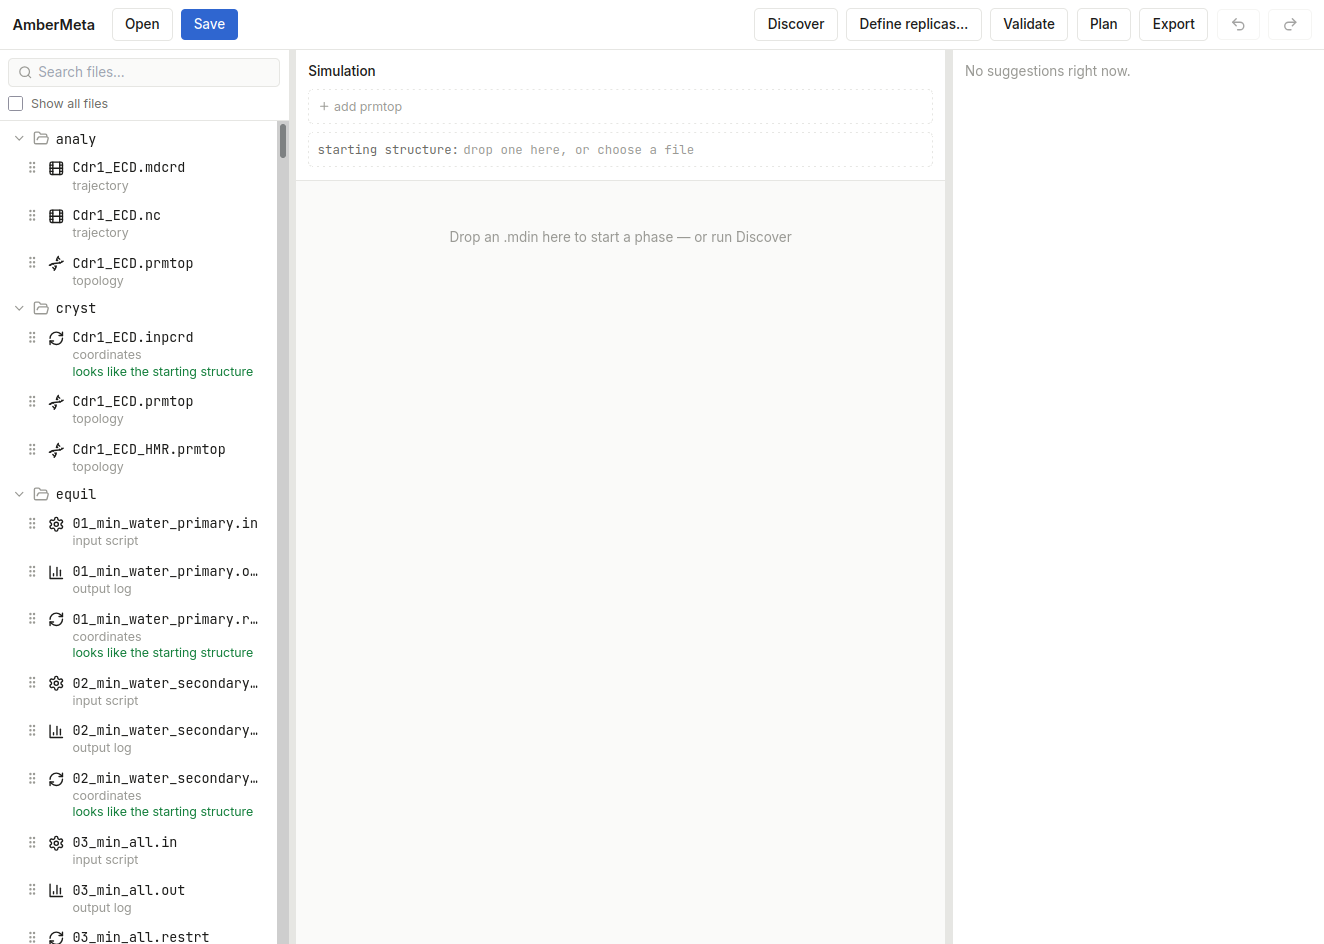
\includegraphics[width=0.86\textwidth]{figures/gui-files.png}
  \caption{The file pane after launching against a system directory. Files are typed on
  sight --- \emph{topology}, \emph{input script}, \emph{output log}, \emph{coordinates} ---
  and candidates for the starting structure are flagged.}
  \label{fig:files}
\end{figure}

\subsection{Discover}

Press \textbf{Discover}. AmberMeta walks the tree, groups files into runs, infers each
phase's role from the inputs, and links each run to the one whose restart it consumed.
The result is a timeline (Figure~\ref{fig:discovered}).

Read down the timeline and check three things:

\begin{itemize}
  \item \textbf{Phase roles.} Minimization, heating, equilibration and production should
        be labelled as such. A phase labelled \emph{Unassigned} usually means a
        preparation step (tLEaP, ParmEd) was picked up as a run --- set its role or
        delete it.
  \item \textbf{The chain.} Between consecutive steps you should see
        \emph{restart of \ldots}. A step reading \emph{starting structure} part-way
        through a production sequence means the link could not be established.
  \item \textbf{Topologies.} Where several topologies exist, check each phase is bound to
        the right one. A repartitioned-mass topology is tagged \textsc{hmr}.
\end{itemize}

\begin{figure}[htbp]
  \centering
  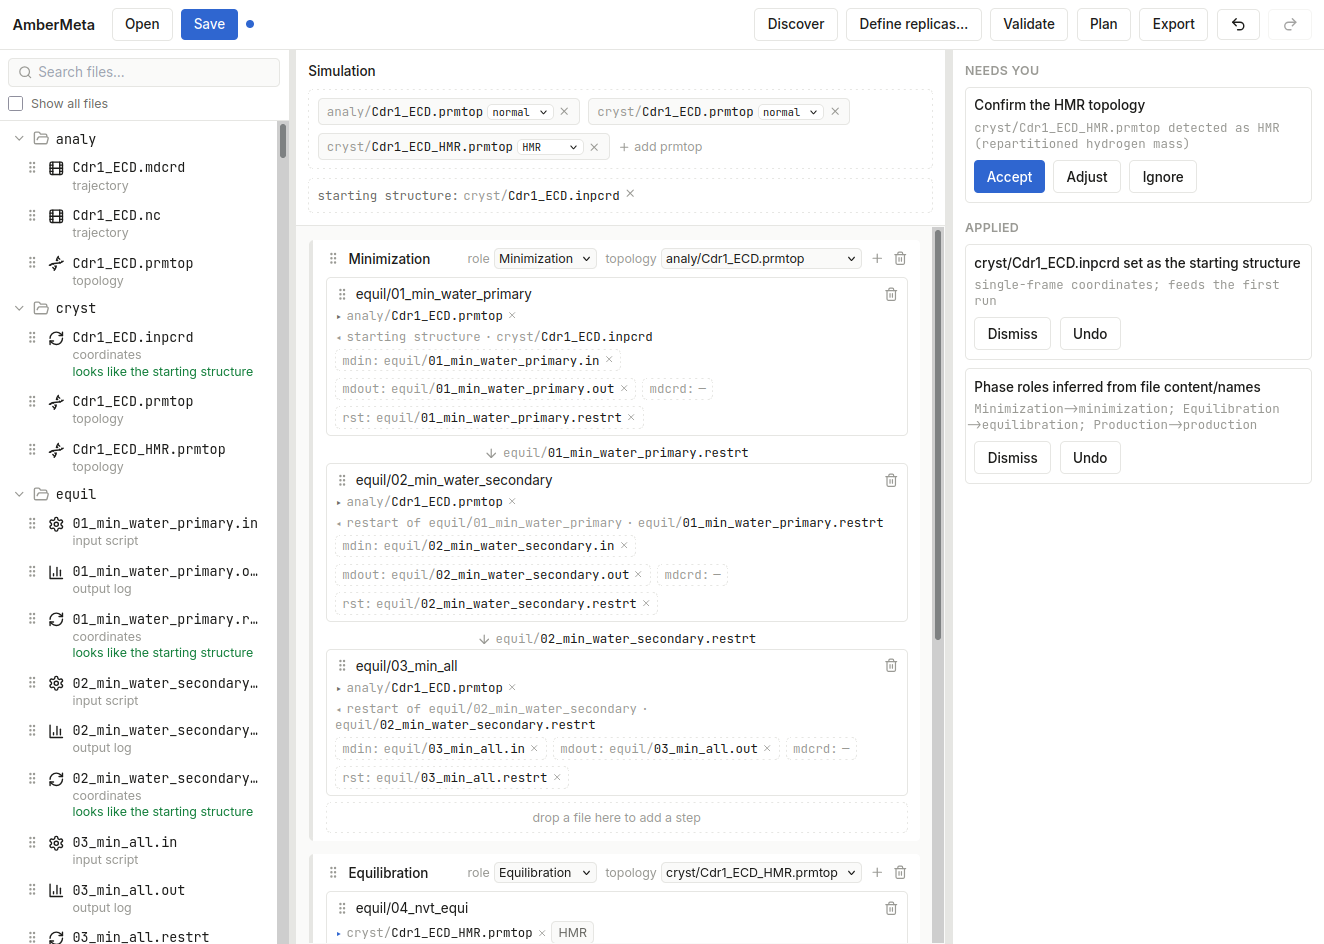
\includegraphics[width=0.86\textwidth]{figures/gui-discovered.png}
  \caption{After \textbf{Discover}. The centre pane is the reconstructed timeline, with
  each run's inputs, outputs and the restart it continues from. The right pane separates
  what AmberMeta did on its own (\textsc{applied}) from what it needs you to confirm
  (\textsc{needs you}).}
  \label{fig:discovered}
\end{figure}

\subsection{Define replicas}

If the system was run as replicas, tell AmberMeta so. Runs in different replicas are
independent trajectories; without this they are treated as one sequence and the
junctions between them are reported as gaps.

Press \textbf{Define replicas\ldots}. If the layout follows \S\ref{sec:layout}, the
members are already proposed --- accept them. Otherwise pick the directory level that
distinguishes the replicas and accept only the members that really are replicas
(preparation directories at the same level are offered too, and should be left alone).

Once accepted, each phase carries a banner naming the member and its run count
(Figure~\ref{fig:replicas}).

\begin{figure}[htbp]
  \centering
  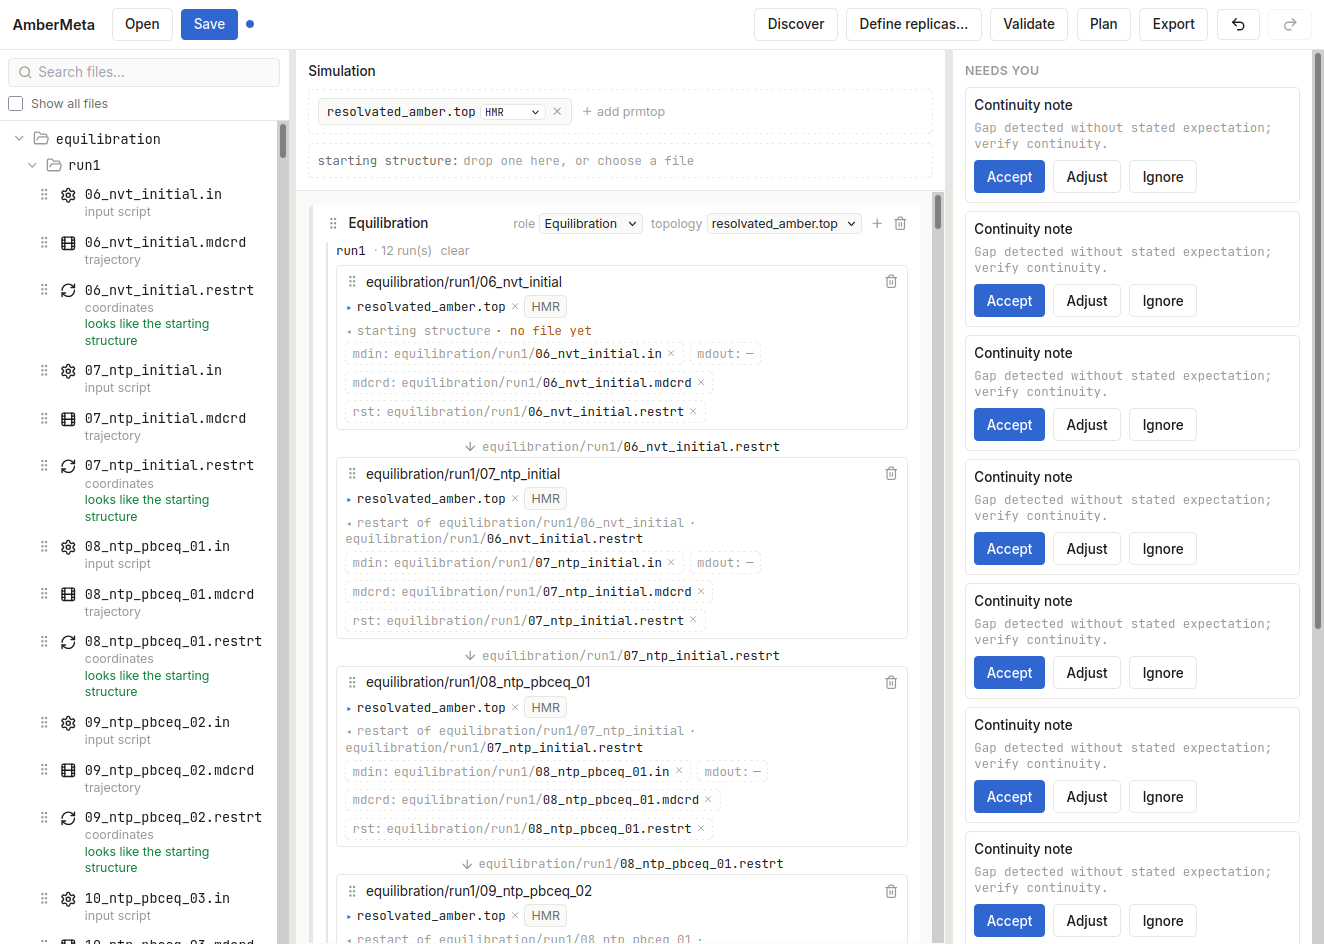
\includegraphics[width=0.86\textwidth]{figures/gui-replicas.png}
  \caption{A system with replicas accepted: the \code{run1} banner above the timeline
  marks the member and its twelve runs. The continuity notes on the right are this
  deposit's missing output logs --- with no \code{.mdout}, no junction can be confirmed.}
  \label{fig:replicas}
\end{figure}

\subsection{Validate, and resolve what it raises}

Press \textbf{Validate}. Findings arrive in the right-hand tray in two groups:

\begin{description}[leftmargin=1.4em,style=nextline,font=\bfseries]
  \item[\textsc{applied}] Inferences AmberMeta already acted on, each with an
        \textbf{Undo}. Skim these --- they are claims about your data. The starting
        structure and phase roles usually land here.
  \item[\textsc{needs you}] Questions it will not answer on its own. \textbf{Accept}
        agrees, \textbf{Adjust} lets you supply the right value, \textbf{Ignore} records
        that you considered it.
\end{description}

\noindent The findings you are most likely to see, and what they mean:

\begin{center}\small
\begin{tabularx}{\textwidth}{@{}l>{\raggedright\arraybackslash}X@{}}
\toprule
\textbf{Finding} & \textbf{What to do}\\
\midrule
Confirm the HMR topology & Check the flagged topology really is the mass-repartitioned one, then accept.\\
Gap detected without stated expectation & Two consecutive runs do not meet in time. Either a run is missing from the deposit, or the gap is real and deliberate --- say which.\\
Atom count mismatch across files & A step is bound to the wrong topology. Rebind it in the timeline.\\
Trajectory is truncated or still being written & The run is incomplete or was copied mid-write. Re-copy it, or accept that its times come from the log instead.\\
\bottomrule
\end{tabularx}
\end{center}

Resolve findings until only ones you have deliberately accepted or ignored remain. A
finding left unresolved is not an error --- it is an unanswered question travelling with
your data.

\subsection{Save}

Press \textbf{Save} to write \code{manifest.yaml} into the system directory. This is the
deposit artifact. \textbf{Plan} additionally writes the summary files
(\code{summary.json}, \code{methods\_summary.json}) used for reporting.

Re-running this procedure later re-reads the files; unchanged files are not re-parsed,
so a second pass over an unchanged system is quick.

\section{Applying this to existing deposits}
\label{sec:existing}

Data already collected does not follow one convention. The four encountered so far, and
what each needs:

\begin{center}\small
\begin{tabularx}{\textwidth}{@{}l>{\raggedright\arraybackslash}p{0.30\textwidth}>{\raggedright\arraybackslash}X@{}}
\toprule
\textbf{Layout} & \textbf{Example} & \textbf{Action}\\
\midrule
Replicas inside each stage & \bpath{equilibration/run1..run6} & Accept the proposal.\\
\addlinespace[2pt]
Numbered replicas in a stage & \bpath{prod/01..05} & Accept the proposal.\\
\addlinespace[2pt]
Replicas beside the stages & \bpath{run1..run4} beside \bpath{equilibration/} & Pick the top level in \textbf{Define replicas\ldots}, then accept only \bpath{run1..run4}.\\
\addlinespace[2pt]
Replica id also in filenames & \bpath{prod/01/GB1_204_01_000} & Pick the replica level manually, then accept only the numbered members.\\
\bottomrule
\end{tabularx}
\end{center}

In the last two cases the automatic proposal is declined rather than wrong: AmberMeta
refuses to guess when a layout admits more than one reading (Figure~\ref{fig:untagged}).
Choosing the level yourself is the intended route, and the resulting manifest is
identical to one from a conforming layout.

\begin{figure}[htbp]
  \centering
  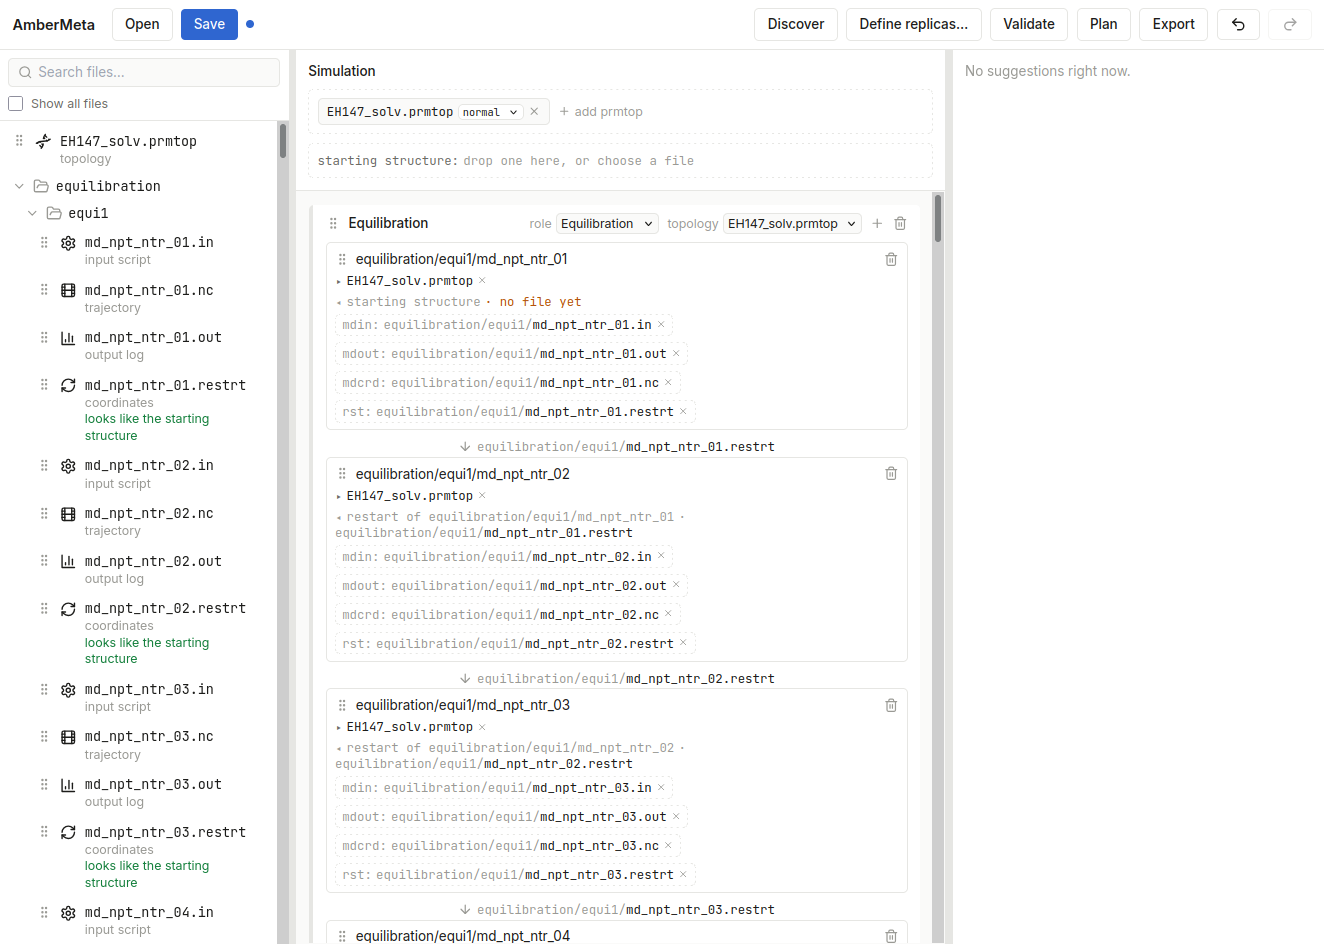
\includegraphics[width=0.86\textwidth]{figures/gui-untagged.png}
  \caption{A layout where replicas were not proposed automatically: the runs are all
  present and correctly chained, but split across many phases with no member grouping.
  \textbf{Define replicas\ldots} is what resolves this.}
  \label{fig:untagged}
\end{figure}

\section{Quick reference}
\label{sec:quickref}

\begin{center}\small
\begin{tabularx}{\textwidth}{@{}l>{\raggedright\arraybackslash}X@{}}
\toprule
\textbf{Step} & \textbf{Command-line equivalent}\\
\midrule
Launch            & \code{ambermeta gui DIR}\\
Discover          & \code{ambermeta discover DIR}\\
Discover + save   & \code{ambermeta discover DIR -{}-write manifest.yaml}\\
Build \& check     & \code{ambermeta plan DIR -{}-recursive}\\
Summaries         & \code{ambermeta plan DIR -{}-recursive -{}-summary-path summary.json}\\
Check one file    & \code{ambermeta validate FILE [FILE \ldots]}\\
Inspect one file  & \code{ambermeta info FILE}\\
\bottomrule
\end{tabularx}
\end{center}

\noindent\small Note that \code{validate} checks individual
files; the whole-campaign check the \textbf{Validate} button performs is what
\code{plan} does while assembling the protocol.\normalsize

\begin{note}{Checklist per system}
\begin{enumerate}[nosep]
  \item Every directory readable; no stray files among the runs.
  \item Output logs present for every run.
  \item Discover run; phase roles and the restart chain read correctly.
  \item Replicas defined, if the system has them.
  \item Validate run; every finding accepted, adjusted or deliberately ignored.
  \item \code{manifest.yaml} saved into the system directory.
\end{enumerate}
\end{note}

\end{document}
